\section{The \sys{} confinement system}
\label{sec:system}

In this section, we describe the \sys{} system.
%
Unlike existing browser security mechanisms, \sys{}'s emphasis
is on providing \emph{confinement:} the ability to give code access to sensitive
data while ensuring that the code cannot release that sensitive
data arbitrarily~\cite{SaltzerS75}.
%
Our confinement mechanism allows developers to enforce both policies
that are stricter than the SOP and policies that are more flexible
than the SOP, while still providing understandable security assurances.

\subsection{Compartments and origins}

The basic unit of confinement in \sys{}---a compartment---corresponds to
a JavaScript execution context, e.g.\@ a browser tab, an iframe on a
page, or even a Web Worker~\cite{workers}.  Both compartments as well as
web sites are associated with security policies which dictate what kind
of messages and requests are permitted to flow with other compartments
and web sites.  This model of a compartment is already prevalent on the
web; however, our security policies are different from the traditional
Same-Origin Policy, which only restricts compartments from reading data
from arbitrary web sites.  We describe our new policy in the next
section.

\subsection{Labels}

The method by which security policies in our system are specified
are using \emph{labels}.
%
Conceptually, a label protects all of the data associated with a
compartment, specifying what origins can read and write the data.
%
The particular labels that are used in \sys{} are \emph{DC
labels}, presented in~\cite{stefan:2011:dclabels}.
%
We chose DC labels, much like Hails~\cite{giffin:2012:hails} and
Breeze~\cite{Breeze13}, because they have a simple and clear
semantics, yet are as expressive as the labels used by other practical
confinement systems~\cite{GenLabels}.

A privacy label (henceforth just label) is a boolean formula over
origins:  intuitively, it specifies what origins can read this data.%
\footnote{
  Our system also handles \emph{integrity}, but it is omitted from
  the discussion for simplicity.
}
%
We sometimes abuse terminology and use the phrase  ``label of a
browsing context'' to mean the label on the compartment that contains
the browsing context's document, even though, for example, Worker
compartments do not have a document or browsing
context~\cite{workers}.
%
By default, the label of a compartment is the origin of the source
website; e.g.\ an iframe hosted by {\tt https://bank.ch} would be
labeled {\tt https://bank.ch}.
%
When a compartment wishes to send a message to another compartment (or
any sort of one-way communication), we check if the target
label logically implies the source label: intuitively, we are checking
that the security of the destination is sufficient to preserve the
original security policy.
%Reworded version: Intuitively, an entity is allowed to receive data that is at most as
%sensitive as its label, i.e., the entity's label always \js|subsumes|
%the label of the data it can receive, preserving the latter's privacy.
\Red{maybe something about how this makes it first
class: the fact that policies are preserved means that if a library has
sub-libraries, they will get the appropriate policy enforced}
%
For example, a compartment labeled ``\https{bank.ch} and \https{amazon.com}''
%\js|Label("https://bank.ch").and("https://amazon.com")|
could contain sensitive data from both origins.
%
%Such a label may be used by an application that compares bank
%statements with Amazon purchases.
%
It can read data from either website, but
it cannot make a request to \https{amazon.com}, since the logical
implication does not hold: rightfully
so, since such a request could leak private information from \https{bank.ch}
to \https{amazon.com}.
%
Conversely, data labeled ``\https{bank.ch} or \https{amazon.com}''
can be passed to either website. \Red{Forward reference to privileges.}
%
\todo{ds}{Maybe note that stylesheets are not compartment but a load
caused by parsing a styleshee also obeys IFC since the stylesheet
has a principal which contains a CSP encoding most of the important
IFC stuff}

% it sort of sounds like this might be handled
%   The implicit label of an end-point is simply \js|Label(|\emph{resource
%   origin}\js|)|.
%   %
%   So, for example, when performing an XHR request to \https{a.com} the
%   label of the end server is considered to be \js|Label("https://a.com")|.
%   %
%   Thus this label must subsume the current label if the request is to be
%   permitted.

%When exchanging information, the actual check performed by \sys{} is
%logical implication, as implemented by the \js|Label| method
%\js|subsumes|.
%
%Specifically, \sys{} ensures that data labeled \js|ldata| can be only sent
%to an entity labeled \js|lentity| if
%\js|lentity.subsumes(ldata)| is \js|true|.
%
%
We refer the interested reader to~\cite{stefan:2011:dclabels} for more
details.

\subsection{Label changes and privileges}

While we have specified that the security policies of compartments
are labels, we have not said how these policies are assigned.  A
compartment can freely choose to \emph{raise} its label (opting
into a more restrictive security policy).
%
For example, a compartment labeled \https{bank.ch} cannot read data
from \https{amazon.com} unless it raises its label to ``\https{bank.ch} and \https{amazon.com}''.
%
This leads to a common interpretation of labels as ``taint;'' as
a compartment reads data from more sources, the sensitivity of the
data it contains increases.

\Red{motivating sentence for privileges}
%
A \emph{privilege} is an unforgeable object with which code can assert the
authority of the corresponding origin, allowing it to declassify
data.
%
In \sys, a browsing context has the privilege corresponding to the
page origin.
%
For example, a script running in an \https{amazon.com} page has the
privilege corresponding to the \https{amazon.com} origin, and
can take data labeled with this origin and make it public.
%
In turn, this privilege is used when performing any \js|subsumes|
label checks.
%
\Red{Examples here are confusing, but basically the right idea}
Without this privilege the script cannot perform any XHR requests
(even to \https{bank.ch}) if the context label is
``\https{bank.ch} and \https{amazon.com}'';
such a conjunctive label cannot be subsumed by an end-point-label, and
in this case, prevents data sensitive to \https{amazon.com}
from being leaked to \https{bank.ch}.
%
However, with the  \https{amazon.com} privilege, the code can perform
XHR requests to \https{bank.ch}; in doing so, it is exercising the
authority over \https{amazon.com} data and effectively declassifying
any \https{amazon.com}-sensitive data used in the request.
 
Importantly, code cannot synthesize arbitrary privileges.
%
For example a script executing in a \https{amazon.com} browsing
context cannot create a privilege for \https{bank.ch} and declassify
arbitrary bank data---this would trivially violate any confinement
guarantees.
%
In our system, code can only create the empty privilege (which is
simply the JavaScript \js|null| value) and privileges corresponding
to fresh, unique origins (created with the \js|FreshPrivilege|
constructor).
%
As in HiStar~\cite{Zeldovich:2006}, the ability to generate fresh privileges
ensures that all browsing contexts are egalitarian, i.e., a child iframe is no
less trustworthy than its containing parent.  Figure~\ref{systemAPI} shows the
API to handle privileges (primitives \js|combine| and \js|asLabel| to be 
explained in the next subsection). 


In an ideal confinement system, code can read arbitrary data at the
cost of raising the context label (and thus giving up write
capabilities).
%
Unfortunately, practical systems typically have covert channels which
may be exploited to leak sensitive data.
%
Hence, as in HiStar~\cite{Zeldovich:2006}, Hails~\cite{giffin:2012:hails}, and
Breeze~\cite{Breeze13} we associate a \emph{clearance}---which is
simply a label---with every compartment.
%
Clearance imposes a limit on the kind of data a compartment can have,
i.e., it is an upper-bound on compartment label, and thus the kind of
data a piece of code executing in the compartment can access.

%   For completeness, we summarize  \sys{}'s API for compartments
%   in Figure~\ref{systemAPI}. In the next subsection, 
%   we explain the purpose of the different primitives through examples. 
%   We remark that \sys{}'s API is designed to be minimalistic, and as such, it only
%   consists on the primitives shown in Figures~\ref{fig:APIspec} and
%   \ref{systemAPI}.

%   In the rest of this section, we expand on the \sys{} design by
%   introducing mechanisms that meet the requirements of the four
%   example applications described in Section~\ref{sec:goals}.
%% through
%% three concrete examples: 
%% a password-strength checker (Section~\ref{sec:system:worker}),
%% a password manager (Section~\ref{sec:system:iframe}), 
%% a third-party mashup (Section~\ref{sec:system:mashup}), and
%% a library that converts phone numbers to links
%% (Section~\ref{sec:system:script}--Section~\ref{sec:system:extension}).
%
%For completeness, we summarize the different system components,
%security mechanisms, and DOM API (using WebIDL-like syntax), in
%Table~\toref{table:components}.

\subsection{Lightweight workers}

% DOM workers (paragraph at the end)

As noted in Section~\ref{sec:goals}, and previously observed
in~\cite{Ingram:2012}, workers are a good first step towards reasoning
about the security implications of untrusted code that does not need
to access the DOM, since they provide a clean, isolated environment
within which untrusted code can be executed.
%
However, workers are constrained by the SOP, CSP, etc.
%
Hence, we extend the Worker DOM API~\cite{workers} with a
Labeled-Worker (LWorker).
%
Like a standard worker, an LWorker executes a piece of code in a fresh
compartment that exposes a limited set of objects and properties.
%
Concretely, we expose the \sys{} API (including the \js|LWorker|
constructor used to construct additional labeled Workers), the \xhr{}
constructor used to perform network requests, and
\js|onmessage|/\js|postMessage| used for communicating with the
parent.
%
Different from the \js|Worker| constructor, the \js|LWorker|
constructor, shown in Figure~\ref{systemAPI}, takes three additional
arguments: a label that specifies the clearance on the code running in
the worker, an optional privilege to grant the worker, and an optional
window object to attach to the worker.
%
We discuss the role of the latter two arguments in
Sections~\ref{sec:system:script} and \ref{sec:system:extension}.

To address these issues, we allow developers to create labeled workers that
have access to the page DOM and page-origin privilege.
%
(We naturally call them \emph{labeled DOM workers}.)
%
As noted in Section~\ref{sec:system:worker}, the \js|LWorker|
constructor can be supplied with a \js|Privilege| and \js|Window|
argument.
%
These arguments, for example, allow \https{bank.ch} to create a labeled DOM
worker that has access to the \https{bank.ch} privilege before completely
confining the page:\footnote{
  Since untrusted code will be executing in the context, we use a
  closure to ensure that the privileges do not escape into the outer
  scope.
}

Of course, allowing a labeled DOM worker to arbitrary inspect and
modify the page is not safe.
%
Notably, when untrusted code is executed in such a worker.
%
Thus, \sys{} mediates all worker DOM access to ensure that no information can
(unsafely) leak between the compartments.
%
Specifically, for all \js|get|, \js|set| and \js|call| operations we
ensure that both the page label subsumes the label of the worker 
and the label of the worker subsumes the page label,
both taking into consideration the worker's privileges.
%
In other words, this requires the label of the worker and page be the same,
when considering the worker's privileges.

\subsection{Labeled blobs}

\section{Applications}
\label{sec:system:worker}

%\para{\sys{} approach}
%
%
%% (Rather today's mechanisms give developers a limited form of access
%% control.)
%
\sys{} allows developers to treat a piece of code as untrusted and
confine it, in turn. This functionality is instrumental in supporting
the password-checker application.
%
We first consider the confinement of untrusted libraries that do not
rely on the DOM; in Sections~\ref{sec:system:iframe} and
\ref{sec:system:extension} we address confinement of third-party code
with access to the DOM.


Using this API, we create a new LWorker that executes the
password-strength checker code and registers a callback to receive the
strength score:
\begin{jscode}
// instagra.me main page ...
var url = "https://checker.biz/checker.js";
var label = new Label(location.origin);
// 1. Execute checker in new worker
var checker = new LWorker(url, label);
// 2. Register handler to get score from checker
checker.onmessage = function(event) {
  var score = event.data; 
  // ...
}
\end{jscode}
%
\sys{} first enables \emph{confinement-mode} and sets the browsing
context label to the public label \js|Label()|.
%
In general, a script enables confinement-mode by using our any part of
API; when implicitly enabling confinement-mode, \sys{} takes a
permissive approach and sets the initial browsing context label to the
public label (much like the SOP).
%
However, scripts can also set the compartment label to a label more
restricting than the initial public, current label.
 
When creating the worker, \sys{} ensures that the page is allowed to
make a request to \js|url| to fetch the source code.
%
As with loading content (e.g., images, styles and scripts), writing to
storage (e.g., cookies), or performing explicit network requests with
\xhr{}, \sys{} asserts that, given the current context privileges, the
label of the resource subsumes the browsing context label.
%
In this case, the resource label \js|Label("https://checker.biz")|
subsumes the context label \js|Label()| and thus fetching the script
is permitted.

Before executing the fetched script in the new worker compartment, \sys{}
ensures that the label of the worker is at least as restricting as the
current label.
%
This check ensures that the page cannot declassify data by laundering
it through a worker whose label is less sensitive than the context
label.
\todo{?}{is this clear to non-IFC experts?}
%
\iffigures
\ifcompletefigures
As shown in Figure~\toref{fig:strength-1}, 
\fi
\fi
\sys{} then starts
executing the checker code in the LWorker; the initial label of the
worker compartment is set to that of the parent (in this case, the
public label).\footnote{
%
Our use of labeled workers in this fashion is similar to LIO's
use of labeled threads~\cite{stefan:addressing-covert}.
%
However, when considering workers that share an event loop this more
closely resembles LIO's \js|toLabeled|
block~\cite{stefan:2011:flexible} and Breeze's
\js|bracket|~\cite{Breeze13}.
}
 
At this point, the code executing in the labeled worker can fetch
data, such as a list of weak passwords from any origin,
CORS-permitting.
%
It is important to note that since the password-strength checker has
not yet read any sensitive data, which is reflected in the compartment
label, this is a safe operation, i.e., making the request does not
leak any information.
%
Only once the code decides to inspect the password should it no
longer be able to perform such arbitrary network requests.

To retrieve the password, the password-strength checker registers a
message-event handler, which is invoked when the parent sends it a
message whose label is subsumed by the checker's label.
%
The checker code is given below.
\begin{jscode}
// checker.js ...
// Assume SWAPI.label == Label()
function computeStrength(pass) { /* ... */ }

// 3. Raise context label & register handler
SWAPI.label = SWAPI.clearance;
// SWAPI.label == Label("https://instagra.me")
onmessage = function(event) {
  var password = event.data;
  // 5. Check score & send it to parent:
  postMessage(computeStrength(password));
};
\end{jscode}
%
Note, that, here, the worker first raises the context label to the
clearance---which is the worker label---by setting
\js|SWAPI.label|.\footnote{
  Alternatively, before raising the current label the worker and
  parent could implement a message-passing protocol that establishes
  to what label the worker should raise its label. For simplicity, the
  worker raises its label to its clearance.
}
%
In doing so, the code is effectively stating that it is ready to
receive data at sensitivity level \https{instagra.me}, at the cost of
giving up arbitrary communication capabilities.
%
The checker can now receive sensitive data (the password), but, for
example, can only use \xhr{} to communicate with \https{instagra.me};
%
performing arbitrary network requests or creating arbitrarily-labeled
workers is no longer permitted.

Next, the page extracts (from the DOM input element) the password and
sends it, via \js|postMessage|, to the LWorker executing the checker:
\begin{jscode}
// instagra.me main page ...
var password = 
 document.getElementById("password").value;
// 3. Send checker password 
checker.postMessage(password, label);
\end{jscode}
Here, \js|postMessage| additionally takes the label of the message
\js|label|, which must be subsumed by both the browsing context
clearance and worker label.
%
(If an explicit label is not supplied, \sys{} uses the browsing
context label as the message label.)
%
We use this label to ensure that the receiver's message handler is
dispatched only if its browsing context label is at least as sensitive
as \js|label|---thus preserving the privacy of the password.

The \js|postMessage| dispatches the worker event handler with the
parent-supplied password. 
%
As shown above, this handler simply invokes the underlying
password-strength checking function \js|computeStrength|, the result
of which is returned to the parent via \js|postMessage|.
%

Finally, the event handler registered by the page is dispatched and
the score is shown to the user.
%
Since SWAPI imposes a symmetric checks, the label of the page must
subsume the message label (which is the worker's compartment label)
for the handler to be dispatched.
%
As described, this is indeed the case, when considering the page
privileges;
%
we rely on the page having ownership of the \https{instagra.me}
privilege to avoid tainting the browsing context before reading the
score from the worker.

%
Unfortunately, using the label that corresponds to the page privilege
in this fashion---to avoid tainting the page to the label the
worker---also means means that our confinement of the checker code is
limited: it does not restrict the worker from using XHR to
self-exfiltrate data to \https{instagra.me} (much like using CSP's
\verb|'self'| directive).
%
Hence, it is important for the page to be able to label the
worker---and thus messages to it---with an origin that does not
correspond to an actual host as to confine the worker, but not force
the page into raising its label.

This is precisely the role of fresh privileges.
%
A fresh privilege corresponds to a unique origin whose scheme is
prefixed by \texttt{x-swapi}; the fake protocol ensures that when the
current label is raised to the label of this origin, the \xhr{}
constructor cannot be used to make actual requests.
%
Hence, to fully confine the password-strength checker we modify the
\https{instagra.me} page to first create a fresh privilege and use the
corresponding label when creating the LWorker.
%
The modified code is shown below.
\begin{jscode}
// instagra.me main page ...
// Create fresh unique privilege
var p = new FreshPrivilege();
// Take ownership of this privilege
SWAPI.privilege.combine(p);
// Get corresponding label:
var label = p.asLabel;
// Use it to confine the worker completely:
var checker = new LWorker(url, label);
// As before ...
\end{jscode}

We remarks that, different from existing approaches, our system
provides a client-side approach to flexibly and fully confining
untrusted code:
%
the strength checker can perform arbitrary XHR until it raises its
label to register the \js|onmessage| handler that will inspect the
sensitive password; from this point on it can only communicate with
the parent---it cannot perform any XHR.
%
This is in contrast to either giving the checker irrevocable network
access (e.g., with CSP's \verb|'self'|) or none at all (e.g., with
CSP's \verb|'none'|).
%
Importantly, our first-class workers and privileges makes security a
first class citizen: not only can the page consider the checker
untrusted, but the checker can itself create fresh privileges and 
LWorkers in which it can execute code it itself does not consider
trustworthy.
%
(Of course, this is also all dictated by \sys{}'s current label,
privileges, etc..)

\todo{ds}{add figure showing checker in action}
\todo{?}{consistent usage of message handler, event handler, and
callback}

\subsection{Cross-iframe confinement}
\label{sec:system:iframe}
%Password manager 

In the password strength-checker application, the \https{instagra.me}
page effectively imposed the requirement that the password-strength
checker discard its network communication capabilities by raising the
compartment label sufficiently high, in order to read the (labeled)
password.
%
This meets the requirement of confining untrusted code that computes
with sensitive data.
%
More generally, however, by associating a label with every browsing
context and restricting read- and write-effects according to it,
\sys{}'s confinement mechanism can give developers a means for
controlling where users' data can flow, even after the data is made
available to untrusted browsing contexts.

%\para{\sys{} approach}
%
With \sys{}, we can leverage confinement to build a password manager
web application that does not force the user to place complete trust on 
any of the participating parties. We use the password manager as a
running example of this use of confinement.
%
Our password manager is divided into two mutually distrusting
components: a management layer (provided by \https{pwd.eff.org})
that interacts with the user, 
%to store and fetch credentials, 
and a storage layer (provided by \https{dropcu.be}) that provides a
simple
%---in effect, labeled---
%A bit confusing describing it at this point
server-side storage API for the
management layer.
%
The mutual distrust between the layers is instrumental---yet, without
confinement not sufficient---to ensuring that neither party can
individually compromise the user's privacy (and would thus have to be
trusted in full).
%

%
Though a user can use such a password manager to store and fetch secrets
directly, for simplicity, we assume that a website, \https{fb.com},
integrates the manager in order to save and retrieve login
credentials, e.g., through a bookmarklet, \footnote{In Section~\ref{sec:implementation} we describe
an untrusted extension system that can be used to inject the
password-manager specific code into the integrator page.  
} as shown in Figure~\toref{fig:manager-s-1}.
%
\begin{figure}
\begin{center}
% I printed out, and it reads well!
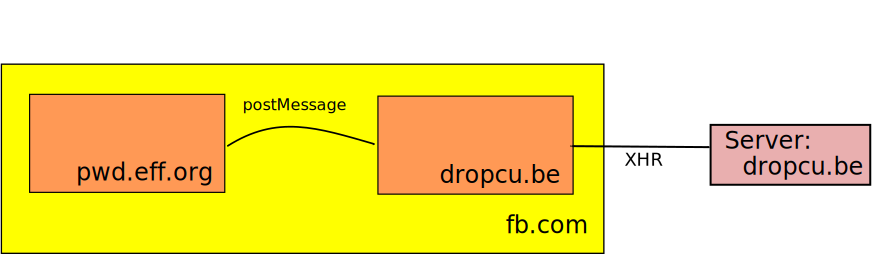
\includegraphics[scale=0.35]{pmanager.pdf}
\end{center}
\vspace{-10pt}
\caption{\label{fig:manager-s-1} Password manager
architecture;\todo{ds}{need better fig}}
\vspace{-10pt}
\end{figure}
%
Without loss of generality, we also assume that encryption and
decryption is carried out on the client-side by the management layer.
%
While some existing storage layers, such as \Red{Mega}~\tocite{},
provide encryption, we require that the encryption and storage layers
be compartmentalized in order to achieve strong security guarantees.
%
These security guarantees and trust assumptions are as follows:
\begin{enumerate}[i)]
\item The management layer never learns the site-specific (\https{fb.com})
  credentials. The user only needs to trust this component with their master
  password. Importantly, without the collusion of the storage layer, the
  management layer cannot exploit the master password in order to reveal
  credentials.

  %
  To eliminate this trust, users can inspect the management layer's
  browsing context label, either using standard developer tools or by
  right-clicking on the page (a functionality implemented by our
  supporting extension, describe in Section~\ref{sec:implementation}),
  and only supply the master password if the label ensures that the
  page cannot disseminate the password arbitrarily.
  %

\item The storage layer never learns the site-specific credentials or
  master password. The user only needs to trust this layer to not
  collude with the management layer (and vice-versa). We believe that
  this is a realistic assumption given a decentralized environment
  like the web.

\item Finally, the integrator never learns the master password or
  credentials private to other websites (e.g., \https{goo.gl}).
\end{enumerate}
%
It is important that the above guarantees be preserved when the
password manager is used to both save and retrieve credentials.
%
Below, we respectively describe the interaction of all the components
in saving and retrieving credentials.

\para{Saving credentials}
%
To save credentials, the integrator, \https{fb.com}, first creates two
iframes: one containing the \https{pwd.eff.org} management layer and
another containing the \https{dropcu.be} storage layer.
%
As part of the initialization process, the management layer saves a
pointer to the storage layer (via \js|window.parent.frames|), both
layers register \js|onmessage| event handlers, and the expected
sensitivity (label) of data to be exchanged is shared.
%
Next, the integrator sends the credentials to the management
layer via \js|postMessage|.
%
The label of the message is
\js|Label("https://fb.com").or("https://dropcu.be")|; this label
ensures that the management layer can only receive the message if it
has raised its context label so that it subsumes the label of the
message, which subsequently limits it to communicating with the
\https{fb.com} and \https{dropcu.be} layers.\footnote{
  To confine the management layer more strictly, the message can be
  labeled with a label corresponding to a fresh origin generated by
  \https{fb.com}, the privilege to which is granted to the storage
  layer. 
}

In general, and as in the LWorker case, the browsing context's
\js|onmessage| handler is only dispatched if the context label
subsumes the message label.
%
This restriction ensures that the browsing context label is
sufficiently strict to protect the privacy of the message.
%
For iframes, when compared to workers), the restriction does not
solely amount to limiting the usage of \js|postMessage| and the \xhr{}
constructor.
%
Rather, \sys{} restricts all network, storage and
cross-browsing-context communication.
%
Specifically, just as sending a \js|postMessage| requires the context
label be subsumed by the message label, as to ensure that sensitive
informatoin from the context is not exfiltrated to less-sensitive
entities, when loading content (e.g., with \js|<img>| or
\js|<script>|), writing to local storage (e.g., with
\js|document.cookie|), performing network requests (with
\xhr{}), or navigating the browsing context, we require that the
context label be subsumed by the implicit label of the resource.
%
This ensures that the action (which is effectively a write) does not
leak any information from the context to a less-sensitive entity.
%
Of course, in all label comparisons, the context privileges are taken
into consideration.
%
 
\todo{ds}{transition to this paragraph needs work}
Returning to our password manager, upon receiving the credentials
\js|credentials| via the \js|onmessage| handler, the management
layer requests the master password (\js|mpass|) from the user, 
generates a \js|salt|, and encryption key $k =
H(\texttt{mpass}\|\texttt{"}\https{fb.com}\texttt{"}\|\texttt{salt})$.
%
Here, $H$ is a hash function such as SHA-256.
%
We use the integrator origin, in addition to the master password and
salt, to ensure that a malicious storage layer will not be able to
confuse the management layer, during the retrieval process, into
decrypting \https{fb.com}'s credentials when invoked by a different
integrator (e.g., \https{goo.gl}).

% 
After the key generation, the management layer encrypts the
credentials using a function \js|E|, such as AES, and sends the tuple
(\js|E|$_k$\js|(credentials)|, \js|salt|) via \js|postMessage| to
the storage layer.
%
Since the management layer's current label---and thus the implicit
message label---is subsumed by the storage layer's current label,
\js|Label("https://dropcu.be")|, the latter's \js|onmessage| handler
will be invoked with the encrypted credentials.
%
We note that, since the storage layer frame has the \https{dropcu.be}
privilege, it does not need to raise its compartment label; this
allows the storage layer to use XHR to send the data to the
\https{dropcu.be} server.
 
We note that, in addition to the credentials and salt, the storage
layer also stores the origin of the parent, i.e., \https{fb.com}, as
meta-data (label) identifying for whom the data is being stored.
%
Rather than having the management layer provide this meta-data to the
storage layer alongside the encrypted credentials, by having
\https{fb.com} create the frame in the initialization stage, we ensure
that a malicious management layer cannot confuse the storage layer
into associating \https{fb.com}'s encrypted data with a different
origin, e.g., \https{goo.gl}, and thus allow it to be leaked during
the retrieval process.\todo{}{Is the above paragragraph clear?}

\para{Retrieving credentials}
%
As in the case of saving credentials, the integrator, \https{fb.com},
creates two frames containing the management and storage layers.
%
In this case, the storage layer first retrieves the encrypted
credentials \js|E|$_k$\js|(credentials)|, salt and ownership meta-data
and registers an \js|onmessage| event handler, that responds to the
management layer's ``fetch'' request.  A simplified handler is shown
below.
\begin{jscode}
function handler(event) {
  // ... check origin ...
  // owner == "https://fb.com"
  // credentials == E_k(...)
  var l = new Label(owner);
  event.origin.postMessage(credentials, l);
} 
window.addEventListener("message", handler);
\end{jscode}
This handler simply replies via \js|postMessage| with the credentials.
%
Importantly, however, the message is labeled with the origin meta-data
retrieved from the server.
%
This ensures that the browsing context label of the frame requesting
the credentials---the management layer---must subsume the label of the
message. 
%
This restriction guarantees that, even if the management layer did not encrypt the
credentials during the save procedure, it cannot learn and
exfiltrate the credentials through this retrieval process; the message
label ensures that it can only disseminate the credentials to the
corresponding owner (\https{fb.com}).
%

Like the storage layer, the management layer also firstly registers a
message handler, though, in this case, to receive the encrypted
credentials. Then, via \js|window.parent.frames|, it retrieves a
pointer to the storage layer, and after raising the compartment label
to \js|Label("https://fb.com")|, it sends the storage layer a
``fetch'' message, requesting the encrypted credentials.
%
This, in turn, leads to the dispatch of the storage layer's handler
(defined above), which replies with a message containing the encrypted
credentials and salt.
%
At this point, the management layer's message handler is invoked
(since the management layer's context label subsumes the label of the
storage layer message).
%
Using the master password, \js|mpass| (that was fetched from the user)
and salt, the management layer reconstructs key $k$ and uses it to
decrypt the encrypted credentials.
%
These decrypted credentials are then sent to the \https{fb.com}
browsing context.
%
We note that, as imposed by the storage layer, the management layers'
context label, \js|Label("https://fb.com")|, prevents it from
disseminating the data to any other origin.
%
Finally, \https{fb.com}, whose label is still public, carries out the
login procedure (e.g., by submitting the login form).

\subsubsection{Generalizing the application}
The design pattern used for the password manager can be exploited in other
scenarios. To illustrate this point, we implemented a prototype of a
mashup capable of handling encrypted on-line documents.
%Companies often argue against using on-line documents services (like Google
%Docs) due to privacy issues, i.e., they do not want Google to store sensitive
%information present in such documents. Using a similar architecture as the
%password manager, we implement a prototype of a mashup capable to handle
%encrypted on-line documents. 
This prototype shows the feasibility of our approach in combining
services such as online document providers (e.g., Google Docs)
and encryption providers. 
%
The goal of the mashup is to allow the user to use a document editor,
while ensuring that the editor-provider can only store encrypted data,
as enforced by an encryption ``provider,'' which is itself confined as
to no leak the documents.
%
Moreover, once encryption keys are configured, the encryption and
decryption should be performed in a mostly transparent manner.

Similar to the password manager, our app prototype relies on three
iframes: an outermost, labeled \js|gdocs.com|, an intermediary encryption
layer, labeled \js|encrypt.com|, and an innermost one labeled
\js|gdocs.com|.
The innermost frame contains the actual document editor (that cannot
communicate with anything except the parent frame), while the middle
layer serves as the encryption mediary between the editor and outer-most
frame that communicates with the \js|gdocs.com| servers.

\todo{}{Can squeeze space by just saying ``token-based auth'' vs.
going into details}
To enforce the aforementioned security policy we use a small
bootstrapping protocol between the middle and innermost frames.
Specifically,
once the middle (encryption-layer) frame is
loaded, it starts an authentication process with the innermost
(editor) frame before any
user input is recorded. To this end, it sends a random token
labeled \js|Label("https://gdocs.com").and("https://encrypt.com")| to
the innermost frame.
This message requires that innermost frame be (at least) tainted with
the described label, and as a result, restricted from performing any network
requests; this ensures that the innermost editor cannot leak
the plain document as it is composed to \js|gdocs.com|. Once the
innermost frame receives this
message, it replies to the encryption layer with the token.
The encryption-layer, in turn, verifies the token, the receipt of which ensures
that the editor-layer is confined---it must have raised its label to
read (and reply with) the token.
At this point, the user is allowed editing the document.

We remarks that saving and restoring documents follows in a similar
fashion to the saving and restoring credentials in the password
manager example.  For example, when saving the document, the plaintext
is sent (via \js|postMessage|) to the middle frame for encryption.
The encryption layer, exercises its privilege \https{encrypt.com} to
send the encrypted document, labeled \js|Label("https://gdocs.com")|,
to the outermost frame, which, in turn, uses XHR to store the document
on \js|gdocs.com| servers. Due to the similarities between the two
applications we do not discuss the encrypted editor further.


\subsection{Privilege separation within iframes}
\label{sec:system:script}

The confinement system presented thus far requires developers to
compartmentalize components/libraries of different trustworthiness into
multiple labeled iframes/workers.
%
%% Though this is sufficient for many libraries and mashups, placing a library
%% such a jQuery, which inherently traverses and modifies many parts of the DOM,
%% in a separate iframe/worker is not practical: developers use jQuery as a
%% JavaScript domain specific language with which they build application.
%
We now return to the \https{bank.ch} example application discussed in
Section~\ref{sec:goals}. How can we ensure that a library such as
jQuery does not leak the user's bank statement?

Rather than attempt to solely confine jQuery within such a page, one
conservative approach we can take is to confine all the code in the
page.
%
To this end, we raise the label of the browsing context and drop the
page privileges before importing the library:
\begin{jscode}
// Raise label:
SWAPI.label = new Label(location.origin);
// Drop privileges:
SWAPI.privilege = null;
\end{jscode}
%
This ensures that the page, independent of jQuery's behavior, can only
disseminate data to \https{bank.ch}.
%
However, this also requires the jQuery library code to be hosted on
the same origin, i.e., \https{bank.ch}.
%

To allow the page to communicate with other domains, the application
must create an iframe to a \https{bank.ch} page, which has the bank
privilege and thus able to communicate arbitrarily with that origin.
%
The role of this child frame is to solely implement the ``trusted''
components of the application.
%
Specifically, its sole role is carry out requests (submitted via
\js|postMessage|) for the parent, after asserting that the request is
safe (e.g., updating local storage to reflect the last page view,
etc.).


Unfortunately, adapting a web page to work with a privileged frame 
is non-trivial for several reasons.
%such compartmentalization is not trivial for 
%realistic scenarios.
%
First, the trusted iframe cannot inspect the DOM (state) of the parent frame
and make decisions based on this state. 
%
(Recall that sometimes confinement is stricter than the SOP.)
%
As a consequence, the frames might need to implement a complicated
message-based protocol to communicate information between them.
%
Second, and more importantly, without knowing a-priori
the URL of the source code, or even the order in which requests should
be made, the privileged frame must decide whether fetching the source
will leak any information---a complex decision we wish to avoid
imposing on developers!  Lastly, the page might need to be adapted
from working with synchronous calls (e.g., changing a DOM element
based on a URL) into working with asynchronous ones; the work
in~\cite{Ingram:2012} already identifies the drawbacks of such a
change in the semantics of web pages.
\todo{ds}{generalize the above examples}


%without falling prone
%to a \emph{confused deputy} attack~\tocite{}.
%
%For example, suppose we wish to ensure that the library cannot carry out
%self-exfiltration attacks.
%
%This, firstly, requires that we set the context label to the label
%corresponding to a fresh privilege.
%
%In turn, we need to grant the privilege to the trusted child iframe
%(as to not restrict it from performing arbitrary requests), and
%request that it fetch the library source code.
%



\begin{jscode}
var tcb =
  (function() {
    var p = new FreshPrivilege(),
    SWAPI.privilege.combine(p);
    // Create worker with privs & DOM access
    var worker = new LWorker("/statement-TCB.js",
                             p.asLabel, SWAPI.privilege, window);
    // Raise label & lower clearance
    SWAPI.label = p.asLabel;
    SWAPI.clearance = p.asLabel;
    // Drop privileges:
    SWAPI.privilege = null;
    // Return new worker
    return worker;
  })();
\end{jscode}
%
\todo{ds}{Do we want to wrap in try-catch?}
%
At this point, the page cannot perform any network communications
(e.g., loading scripts, images, or using XHR).
%
Importantly, however, the labeled DOM worker has access to the window
object and can thus modify the DOM to insert a \js|script| element
that loads jQuery, embed an image, for instance, from
\https{gravatar.com} that may require leaking the hash of the user's
name, etc.
%
Moreover, the code executing in the page can use the ``injected''
jQuery library and implement its functionality as before.
%
Different from the iframe approach with this approach, \https{bank.ch}
does not need to implement a complex protocol between the code
executing in the page (which we treat as untrusted) and the trusted
layer that can perform arbitrary network request---the labeled worker
can directly inspect and modify the DOM and has the privilege to fetch
arbitrary resources.

%
In the above example, the bank \js|tcb| worker is able to inspect and
modify the DOM because the effective label of the worker equals that
of the parent page.\footnote{
%
Here, we are conservative in treating every DOM access as
having both a read and write effect;
%
this is because both \js|get| and \js|call| may respectively call a getter or
function that modifies state.
%
Though accessing a data property as opposed to an accessors property
can be used to distinguish between read-only and read-write
\js|get|s~\cite{ecma}, having consistent semantics is simpler,
despite being more conservative.
}
%


\subsection{A cross-browser extension system}
\label{sec:system:extension}

While the above design pattern is well-suited for confining complex libraries
such as jQuery, for many libraries, compartmentalizing the application by
placing trusted code in a labeled DOM worker and confining the main
page may be too conservative.
%
For example, if \https{bank.ch} wishes to integrate a simple
third-party library that traverses the DOM to convert phone numbers to
links (which we call \emph{Phone2Links}), it is sufficient to execute
the Phone2Links code in an unprivileged labeled DOM worker.
%
This allows the library to do its job---inspecting and modifying the
DOM---without requiring the page to drop its privileges.
%
In fact, the page need only raise the browsing context label from
public to \js|Label(document.location)| to ensure that the untrusted
library---which does not have the page privilege---cannot both read
the page content and use XHR to communicate with arbitrary hosts.
%
Of course, if the bank page does not contain sensitive information
(since sensitive statements may included in labeled iframes) then the
library is allowed to, for example, fetch addresses corresponding to
phone numbers (as to help users lookup up local branches).
%
Though we do not expand on this further, we remark that \sys{} also
allows pages to ``attach'' the \js|document| object after it was
created, and thus allow the worker to fetch any resources
\emph{before} accessing the page's sensitive DOM.

\todo{pm}{note on script injection}

Such use of labeled DOM workers is similar to the content-script
extension model pioneered by Chrome and, more recently, adopted by
Firefox~\cite{Carlini:2012}.
%
The code executing in the untrusted labeled DOM worker is akin to
to current content-script extensions.
%
Thus our system can be used to implement light-weight extensions by
simply executing each ``extension'' in a labeled DOM worker, for each
page.
%
There are, however, two core difference between our approach and
existing ``real'' extensions.
%
Frist, we enforce confinement for light-weight extensions, while
content-scripts are subject to all-or-nothing DAC policies.
%
Second, our extensions do not have access to any privileged
APIs---indeed since they execute in the page---while, while existing
extensions do.

The benefits of confinement for extensions are at least as appealing
as that of web apps, and previously considered in~\tocite{},
%
It it worth noting that although we do yet not support privileged
APIs, and thus cannot re-implement all types of extensions as web
applications,\footnote{
  Though we do not believe this to be a fundamental issues, since
  previous efforts (e.g.~\cite{flume}) have considered labeled
  filesystems, sockets, etc., we belive that extending the
  implementation to consider these APIs is outside the scope of this
  paper.
}
existing extensions that rely only on content scripts can be easily
ported to \sys{}.
%
This not only removes the unnecessary trust placed on such extensions
but further makes extensions portable across browsers.
% 
As a first step towards this goal goal, we implemented an extension
management system (as a real extension) that injects labeled DOM
workers (containing the extension code) into pages whose origins are
approved by the user (at install time).
%


\subsection{Relaxing SOP for confined code}
\label{sec:system:mashup}
%Third-party Mashup
%
\sys{} restricts the communication capabilities of a browsing context
once it has read sensitive data.
%
As envisioned in~\cite{yang:2013:towards}, by equipping the browser with such
confinement mechanism we can now also safely relax the SOP.
%
This relaxation, in turn, allows developers to build applications that access
cross-origin data---in a safe manner and without server-side support---to build
applications that are not otherwise possible today.
%
As an example, consider the third-party mashup scenario.

In a third-party mashup, a party, such as \https{mint.biz},
incorporates user-sensitive data from unaffiliated origins, such as
\https{bank.ch} and \https{amazon.com}, in order to present users with new
interfaces or functionality.
%
For instance \https{mint.biz} may wish to present the user with a
visualization of their spending habits, identify fraudulent
\https{amazon.com} purchases using their \https{bank.ch} account, etc.
%
Currently, such applications cannot be built without sharing (their
\https{bank.ch} and \https{amazon.com}) credentials since the SOP
prevents \https{mint.biz} from accessing the users' \https{amazon.com}
and \https{bank.ch} data, e.g., with \xhr{}.\footnote{
 We assume that neither \https{amazon.com} nor \https{bank.ch}
 explicitly trust \https{mint.biz}; otherwise, the parties can
 explicitly set CORS headers~\cite{cors13} to grant \https{mint.biz}
 access to such data.
}
%
In contrast, \sys{} is able to allow \https{mint.biz} to access such
data, provided that once the data is inspected the page cannot
arbitrarily exifiltrate it (e.g., by performing a network request or
writing to storage).
 
To this end, we modify the \xhr{} constructor to add an additional
flag that indicates whether the object should be treated as an
(implicitly) labeled XHR object.
%
When set, the  label of the object corresponds to the origin
to whom the request is being made (set with the \js|open| method). 
%
Hence, accessing the object state, including the response, is dictated by
confinement, not SOP.
%
Moreover, we ensure that when accessing any of the methods or
properties of the object, any underlying read- and write-effects do
not violate the confinement guarantees provided by the context label.
%
For example, when calling the \js|send| method, which performs the
actual network request, \sys{} checks that the (implicit) label of the
remote origin, to whom the request is being sent, subsumes the current
context label;
%
this ensures that performing the request does not leak any
information.
%
Similarly, when accessing any of the response attributes (e.g.,
\js|status|, \js|responseText|, etc.), \sys{} ensures that the
browsing context can inspect (read) the state of the XHR object which
may contain data from the remote host.
%
Specifically, it checks that the browsing context label subsumes the
label of the XHR object.
%
Finally, and as in the case of dispatching \js|onmessage| handlers,
%between labeled browsing contexts, 
when dispatching any registered XHR
handlers (e.g., \js|onabort|, \js|onload|, etc.), \sys{} also ensures
that the context label subsumes the label of the XHR object, i.e., it
can observe the presence of the message.
 
Note that our modified a XHR object allows the response of a
cross-origin request to be inspected, regardless of the CORS headers;
though more flexible than the SOP, this is is safe since the
inspection of a response raises the context label, and thus restricts
all subsequent side effects.\footnote{
  To avoid unnecessary tainting, this labeled XHR should not be used
  when a resource is expected to have a CORS header that would permit
  the read.
}
%
In our mashup application, once \https{mint.biz} inspects the
response of an \https{amazon.com} request, it cannot perform requests
to any origin other than \https{amazon.com}.
%
Further inspecting a response from \https{bank.ch} leads to a scenario
in which no additional requests can be made: the context label  
\js|Label("https://amazon.com").and("https://bank.ch")|
cannot be subsumed by any origin label. 
% in order to 
% to inspect the response.
%
However, data in the browsing context can still be shared with labeled
frames and workers which may use it in complex ways; \sys{} ensure
that the privacy of the data is preserved.
%whose context labels preserve the privacy described by 
%\js|Label("https://amazon.com").and("https://bank.ch")|.
% %ensures that the privacy of the will be preserved.
% 

Such sharing is important since it allows us to build applications
that retain their ability to perform cross-origin requests across the
lifetime of a page.
%
For example, in our third-party mashup we create two labeled contexts
that use the labeled XHR constructor according to user input, one
communicating with \https{amazon.com} and another with
\https{bank.ch}.
%
The data is is combined in a third iframe (labeled
\js|Label("https://amazon.com").and("https://bank.ch")|.
%
All the frames are contained in a public parent page,
which performs all the navigation and conveys (through messages)
the user input (e.g., ``get next statement'') to the first two
labeled contexts.




% Local Variables:
% TeX-master: "main.ltx"
% TeX-command-default: "Make"
% End:
